\documentclass[11pt, a4paper, titlepage]{article}
\usepackage[left=1.5cm,text={18cm, 25cm},top=2.5cm]{geometry}
\usepackage[utf8]{inputenc}
\usepackage[czech]{babel}
\usepackage{hyperref}
\usepackage{amsmath}
\usepackage{graphicx}
\usepackage{wrapfig}
\usepackage{caption}
\usepackage{subcaption} % add sub figures

% \usepackage{subfig}
% \usepackage{color}
% \usepackage{times}
% \usepackage[bf]{caption}
% \usepackage{hyperref}
% \usepackage[all]{hypcap}
% \usepackage{graphicx}
% \usepackage{url}
% \usepackage[all]{hypcap}
% \hypersetup{colorlinks=false, linkbordercolor=1 1~1, citebordercolor=1 1~1}
% \usepackage[right]{lineno}
% \usepackage{listings}
% \renewcommand\linenumberfont{\normalfont\tiny\color{blue}}

\iflanguage{english}{
    \renewcommand{\uv}[1]{``#1''}
}

% \title{Editory digitální fotografie}
% \subtitle{FYO - Fyzikální optika}
% \author{Petr Fusek <xfusek08@stud.fit.vutbr.cz>}
% \date{\today}


%--------------------------------------------------------------------------------


\begin{document}
\begin{titlepage}
    \begin{center}
        \textsc{\LARGE Fakulta informačních technologií}\\
        \vspace{0.1 cm}
        \textsc{\LARGE Vysoké učení technické v~Brně}\\
        \vspace{\stretch{0.39}}
        {\Huge FYO -- Fyzikální optika}\\
        \vspace{\stretch{0.01}}
        {\huge Editory digitálních fotografií}
        \vspace{\stretch{0.62}}
    \end{center}
    \begin{center}
    \Large
    Petr Fusek \\
    xfusek08@stud.fit.vutbr.cz \\
    \today
    \end{center}
\end{titlepage}


\section{Úvod}
První myšlenka digitální fotografie, byla v~podobě \uv{telefotografie}.
Shelford Bidwell, byl kolem roku 1880 schopen zakódovat obrazové informace pomocí elektrických signálů, které posílal pomocí telegrafu.
Na druhé straně bylo zařízení, které obraz rekonstruovalo řádek po řádku vypalováním obrazových bodů do papíru napuštěného draslíkatým roztokem.
V~roce 1957 Russell Kirsch digitalizoval fotku svého syna a~uložil jí v~malém digitálním souboru na jednom z~raných počítačů.
V~roce 1068 byl sestrojen první senzor, který jako první ukládat světelná data přímo v~digitální podobě, na základě této technologie byla v~rove 1973 postavena první digitální kamera, schopna ukládat obrázky o~rozlišení 0.8 megapixelů.
\cite{first_digital_photography}
 
První digitální veřejně dostupné digitální fotoaparáty se začali objevovat začátkem devadesátých let a~spolu ss nimi výrobci dodávali software, který umožňoval z~fotoaparátu obrázky stáhnout a~dokonce i~upravovat.
První digitální editor ovšem byl součástí digitálního scanneru \uv{Barneyscanner} z~roku 1989, který mohl být použitý k~digitalizaci klasických fotografií a~jejich úpravám.
Tento editor se posléze začal prodávat separátně pod jménem \emph{Adobe Photoshop}.
Photoshop je dnes synonymem pro digitální manipulaci obrázků a~dominuje tento stále rostoucí trh. \cite{digital_editing_histroy}

V~dnešní jsme si zvykli na základní úpravy obrázků do takové míry, že možnost změnit vlastnosti jako je velikost, jas, kontrast, teplota barev apod., jsou standardem pro jakýkoliv software pracující, nebo jen zobrazující digitální fotografie.
V~této práci se zaměřím na základní teorii a~matematiku schovanou pod některými dobře známými posuvníky.
Například jak a~co je gamma korekce, jak naprogramovat barevný filtr a~proč teplotu barev upravujeme v~kelvinech.

\section{Barva a~digitální obraz}
Každý článek o~barvě začíná její definicí jako vjemový zážitek způsobený dopadajícím světlem o~vlnových délkách cca od 400\,nm to 700\,nm, pokračující popisem lidského oka (viz, \cite{wiki:Color},\cite{mul_opora}).
Co je důležité si z~těchto poznatků odnést je, že pořizování, reprezentace v~počítači a~reprodukce barevných obrázků ve všech případech vychází z~toho, jak lidské oko a~mozek reprezentuje barvy.

RGB model, který je používaný v~monitorech pro reprodukci obrazu, je kombinace množství červeného (R), zeleného (G) a~modrého (B), což více méně odpovídá citlivostem 3~barvo-citlivých buněk na sítnici oka.
Na co je ale sítnice nejcitlivější je intenzita dopadajícího světla a~citlivost se mění pro každou barvu.
Proto intenzita každé složky je nějak empiricky navážena a~manipulace s~nimi či transformace do jiných barevných prostorů jsou otázkou rozsáhlých standardů \cite{wiki:Color_space}.
   
\subsection{Barevné prostory a~modely} \label{color_spaces}
\emph{Barevný prostor} je způsob jakým organizujeme barvy, tak aby jeden bod tohoto prostoru odpovídal jedné konkrétní barvě.
Referenčním standardem je barevný prostor \emph{CIELAB} ($L^*a^*b^*$), který obsahuje všechny barvy, které je lidské oko teoreticky schopno rozeznat \cite{wiki:CIELAB_color_space}.

\emph{Barvený model} je potom matematická abstrakce (množina hodnot), které mapujeme na barevný prostor, který je většinou podmnožinou prostoru referenčního.
Tyto prostory potom slouží jako standard pro kalibraci zobrazovacích a~zaznamenávacích zařízení \cite{wiki:Color_space}.

\subsubsection{RGB}

\begin{wrapfigure}[6]{r}{4.5cm}
    \centering
    \vspace{-1cm}
    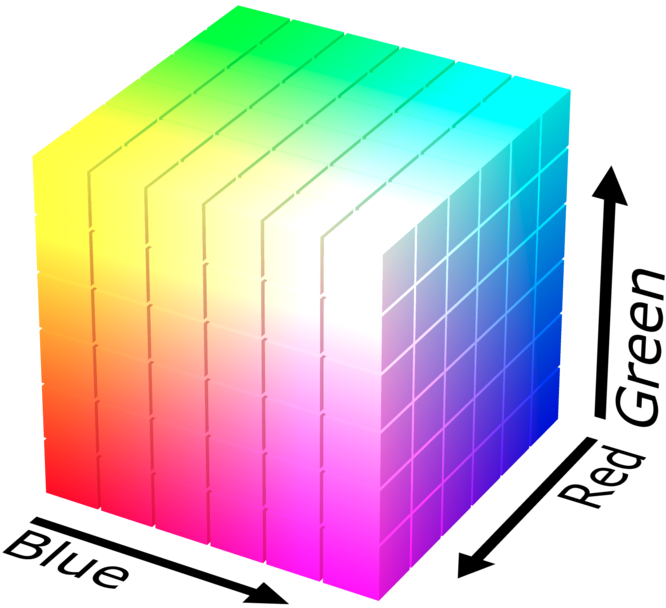
\includegraphics[width=3cm]{RGB_cube.png}
    \caption{RGB prostor \cite{wiki:RGB_color_model}}
\end{wrapfigure}

RGB je asi nejrozšířenější barevný model reprezentovaný jako uspořádaná trojice $(R,G,B)$ hodnot.
Standardizované barevné prostory založené právě na trojicích RGB jsou třeba \emph{Adobe\,RGB}\footnote{\url{https://www.iso.org/standard/45115.html}} nebo \emph{sRGB}\footnote{\url{https://webstore.iec.ch/publication/6169}}.

Popisuje množství světla určitých frekvencí, kterým musí být osvícena sítnice, tak aby jsme jej vnímali jako konkrétní barvu.
Čím více světla (hodnoty) v~každé složce tím více se blížíme bílé barvě.
Světlo se takto sčítá a~hovoříme o~modelu \emph{aditivním}.


\subsubsection{Y$\text{C}_\text{b}\text{C}_\text{r}$}
\begin{wrapfigure}[12]{r}{5cm}
    \centering
    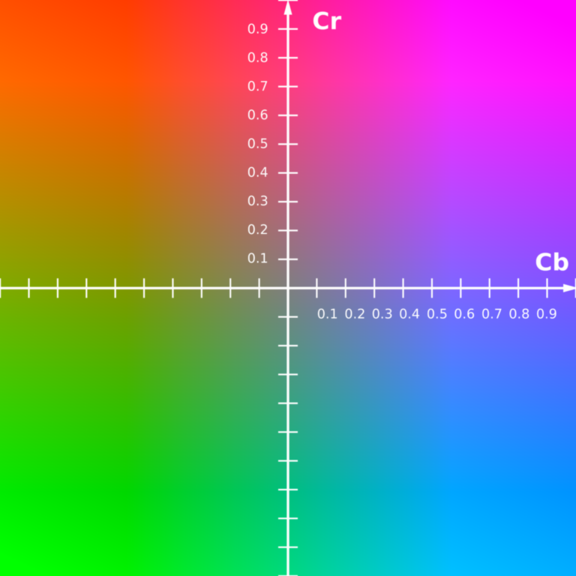
\includegraphics[width=4cm]{YCBCR.png}
    \caption{$\text{C}_\text{b}\text{C}_\text{r}$ výřez při $Y=0.5$ \cite{wiki:YCbCr}.}\label{wrap-fig:1}
\end{wrapfigure}
Model Y$\text{C}_\text{b}\text{C}_\text{r}$ byl vyvinut pro televizní přenosy obrazového signálu, který musel být zpětně kompatibilní s~černobílými televizory.
Využívá právě citlivosti na jas lidského zraku a~většina informací a~detailů je uchována v~jasové Y~složce, čili při zpracování pouze Y~informace dostaneme obraz černobílý.
Složky $\text{C}_\text{b}$ a~$\text{C}_\text{r}$ složí k~posunu jasové informace směrem k~jedné z~barev.
Jasová složka se technicky nazývá \emph{luma} a~z RGB modelu ji lze vypočítat navážením
barvených složek podle empirických citlivostí lidského oka na jednotlivé barvy \cite{mul_opora}:
$$
\begin{bmatrix}Y\\C_r\\C_b\end{bmatrix}
=
\begin{bmatrix}0\\128\\128\end{bmatrix}
+
\begin{bmatrix}
    0,\!299 & 0,\!587 & 0,\!114 \\
    -\,0,\!16875 & -\,0,\!33126 & 0,\!5 \\
    0,\!5 & -\,0,\!41869 & -\,0,\!08131 \\
\end{bmatrix}
\cdot
\begin{bmatrix}R\\G\\B\end{bmatrix}
$$
Výše uvedené koeficienty jsou navrženy pro rychlý přepočet při televizním vysílání, existuje celá škála různých koeficientů pro různé standardy a~formáty s~různými přesnostmi \cite{wiki:YCbCr}.

\subsubsection{HSL a~HSV}
HSL a~HSV modly reprezentují intuitivní míchání barev, a~byly vytvořeny, tak aby si uživatel mohl zvolit jak \uv{saturovaná} či jak \uv{světlá} vybraná barva bude.
Prostory jsou v~obou případech válce, kde H~představuje úhel pootočení kolem jeho osy a~tím se zvolí odstín barvy.
S~označuje vzdálenost od osy válce, která symbolizuje saturaci barvy.
L~nebo V~jsou hodnoty jak vysoko se nacházíme s~tím, že L~představuje světlost (maximální L~se rovná bílé) a~V \uv{sílu} zvoleného odstínu (maximální V~je maximálně saturovaná barva) viz obrázek \ref{fig:hsv_hsl}.
\begin{figure}[h]
    \centering
    \begin{subfigure}[b]{0.3\textwidth}
        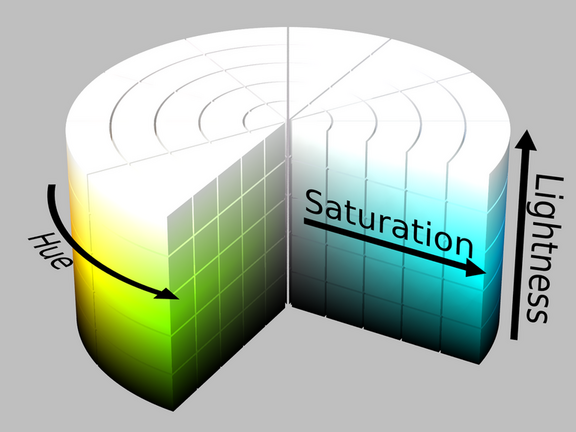
\includegraphics[height=4cm]{HSL.png}
        \caption{$HSL$}
        \label{fig:hsv_hsl:hsl}
    \end{subfigure}
    \hspace{0.2cm}
    \begin{subfigure}[b]{0.3\textwidth}
        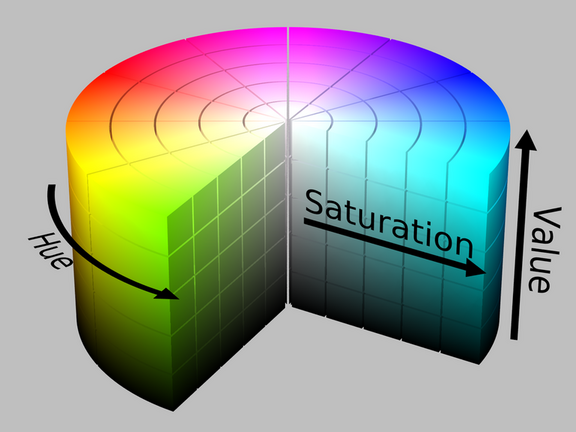
\includegraphics[height=4cm]{HSV.png}
        \caption{$HSV$}
        \label{fig:hsv_hsl:hsv}
    \end{subfigure}
    
    % 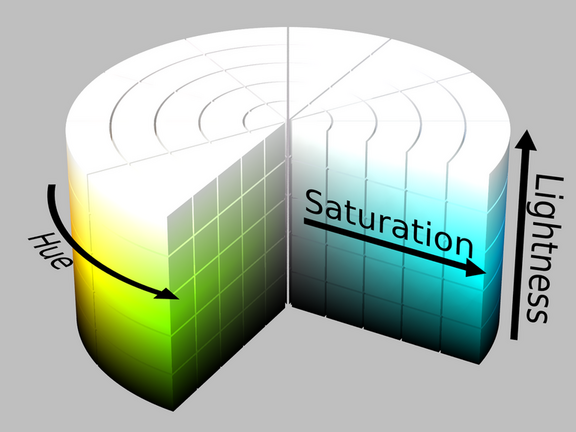
\includegraphics[height=4cm]{HSL.png}
    \caption{Barevné válce \cite{wiki:HSL_and_HSV}}
    
    \label{fig:hsv_hsl}
\end{figure}

\subsection{Reprezentace obrazu v~počítači}
Existuje mnoho způsobů jak ukládat obrazová data v~lineární paměti počítače.
Obrázek je dvourozměrná matice (nebo chcete-li funkce $f(x,y)$), kde jedna hodnota se nazývá pixel (picture element).
Pixely body z~nějakého barevného model (viz. \ref{color_spaces}), nejčastěji RGB, tedy 3~hodnoty, kde $(0,0,0)$ udává barvu černou a~$(\text{\small MAX}, \text{\small MAX}, \text{\small MAX})$ barvu bílou.
jednotlivé barevné složky se nazývají subpixely a~jejich hodnota \uv{$\text{\small MAX}$} je dána počtem bytů, na kterém složky chceme reprezentovat.
Hodnotám subpixelů je nejčastěji rezervován jeden bajt (8 bitů) čili celočíselné hodnoty z~intervalu $\langle0;255\rangle$.
Vzniká tak prostor čítající $256^3 = 16\,777\,216$ možných barev, což je pro běžného člověka dostatečné množství.
Pokud jsou jednotlivé hodnoty v~pamětu uloženy těsně za sebou v~pořadí R-G-B, vychází na jeden pixel 24 bitů a~značíme jaj jako pixel o~formátu RGB24.
Existuje celá řada formátů jejichž označení vypovídá o~jejich rozložení a~velikosti v~paměti (RGB555, BRG24, RGBA32\footnote{A složka označuje alfa kanál, který přižazuje míru průhlednosti pixelu.}, ...) \cite{mul_opora}.

Takto nekomprimovaná obrazová data jsou v~sérii pixel po pixelu uloženy v~paměti nazývané \emph{framebuffer}.
Obrázek má definovaný počet sloupců a~počet řádků.
Jsou očekávávatelně sekvence pixelů jdoucí jsoucí za sebou ale v~paměti mohou být řádky uspořádané shora dolů nebo zespodu nahoru.
Mezi řádky se rovněž vkládá \emph{padding}, tak aby jejich začátky byly zarovnané a~adresovatelné pro rychlejší přístup k~paměti (rozložení můžete vidět na obrázku \ref{fig:framebuffer}).

\begin{figure}[h]
    \centering
    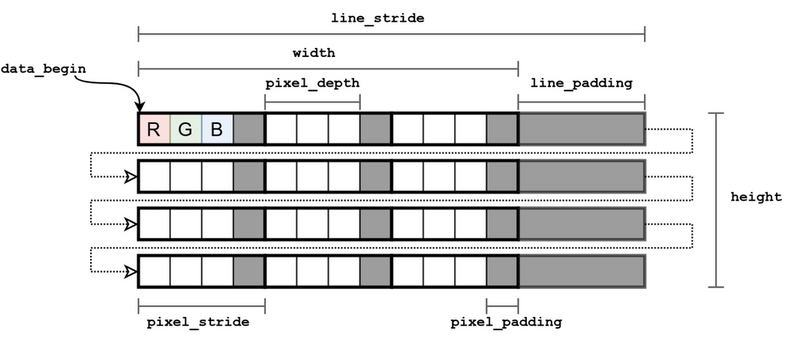
\includegraphics[width=0.9\textwidth]{framebuffer.png}
    \caption{Rozložení framebuffer v~paměti \cite{Whatdoes20:online}}
    \label{fig:framebuffer}
\end{figure}

S~takto uloženými daty je možno libovolně manipulovat a~zobrazovat je uživateli.
Pro jejich ukládání se volí různé kompresní formáty, které jsou mimo záběr této práce.
Editor ovšem musí vždy takový komprimovaný obrázek umět načíst ze souboru do nekomprimovaného framebufferu a~po provedených změnách jej v~komprimované podobě zase uložit. Velkost nekomprimovaného  framebufferu je z~pravidla řádově větší než velikost komprimovaných dat.
Nejpoužívanějším formátem pro ukládání fotografií je \emph{JPEG}, který provádí ztrátovou kompresi a~pro bezztrátovou kompresi obrázků s~omezenou paletou barev se využívá například formát \emph{PNG}.

\section{Operace nad obrázky}
Tato sekce je zaměřena na různé operace, které se s~pixely ve framebufferu nejčastěji provádějí, otevře-li uživatel libovolný editační nástroj.
\subsection{Jas}
\subsection{Kontrast}
\subsection{Teplota barvy}
\subsection{Tónování}
\subsection{Rozmazání a~Filtrace}
\section{Implementace}
\subsection{Technologie}
\subsection{Běžné operace}
\subsection{Demonstrace obecné barevné transformace}

\section{Závěr}

\newpage

\bibliographystyle{alpha}
\begin{flushleft}
  \bibliography{project}
\end{flushleft}

%\appendix
%\newpage
%\section{}

\end{document}
